  \documentclass[12pt]{exam}
\usepackage{amsthm}
\usepackage{libertine}
\usepackage[utf8]{inputenc}
\usepackage[margin=1in]{geometry}
\usepackage{amsmath,amssymb}
\usepackage{multicol}
\usepackage[shortlabels]{enumitem}
\usepackage{siunitx}
\usepackage{cancel}
\usepackage{graphicx}
\usepackage{pgfplots}
\usepackage{listings}
\usepackage{tikz}
\usepackage{circuitikz}
\usepackage{float}


\pgfplotsset{width=10cm,compat=1.9}
\usepgfplotslibrary{external}
\tikzexternalize

\newcommand{\class}{Electronica para Ciencias} % This is the name of the course 
\newcommand{\examnum}{PreInforme Experimento 4 - Sesion 1} % This is the hame of the assignment
\newcommand{\examdate}{\today} % This is the due date
\newcommand{\timelimit}{}





\begin{document}
\pagestyle{plain}
\thispagestyle{empty}

\noindent
\begin{tabular*}{\textwidth}{l @{\extracolsep{\fill}} r @{\extracolsep{6pt}} l}
	\textbf{\class} & \textbf{Name:} & \textit{Sergio Montoya}\\ %Your name here instead, obviously 
	\textbf{\examnum} &&\\
	\textbf{\examdate} &&
\end{tabular*}\\
\rule[2ex]{\textwidth}{2pt}
% ---

\begin{enumerate}
  \item Circuitos:

    \begin{figure}[H]
      \begin{center}
        \begin{circuitikz}
         \draw(0,0)
	 to[V, v= $0/5$](0,2)
	 to[R= $10k$ ](2,2)
	 to[C=$100nf$ ](2,0)
	 to[short](0,0);
	 \draw(2,2)
	 to[short](2,3)
	 to[short](4,3);
	 \draw(0,2)
	 to[short](0,4)
	 to[short](4,4);
        \end{circuitikz}
      \end{center}
      \label{fig:Circ41}
    \end{figure}

    \begin{figure}[H]
      \begin{center}
        \begin{circuitikz}
          \draw(0,0)
	  to[V, v=$0/5$ ](0,2)
	  to[R=$100$ ](2,2)
	  to[C=$1\ uF$ ](2,0)
	  to[short](0,0);
	  \draw(2,0)
	  to[short] node[ground] {} (6,0)
	  to[L=$470\ uH$ ](6,2)
	  to[short](2,2);
	  \draw(6,0)
	  to[short](8,0)
	  to[R=$2k$ ](8,2)
	  to[short](6,2);
	  \draw(0,2)
	  to[short](0,4)
	  to[short](10,4);
	  \draw(8,2)
	  to[short](10,2);
        \end{circuitikz}
      \end{center}
      \label{fig:Circ42}
    \end{figure}
  \item En este caso la constante del tiempo del circuito $RC$ es justamente la multiplicación entre el valor de $R$ y el de $C$ y dado que vamos a hacerlo con el circuito \ref{fig:Circ41} entonces su valor es: \[
      R\cdot C = 10k \cdot 100 = 0.001s
  .\] 

  Ahora bien, para el voltaje instantaneo tenemos: \[
    V_{inst}=V_0\left( 1-e^{-\frac{t}{\tau}} \right) 
  .\] que en este caso debemos considerar que la fuente es una $AC$. Sin embargo, esta es de solo 50Hz. Por lo tanto, cada ciclo dura aproximadamente $0.02 s$ cuando $\tau=0.001$ por lo tanto no alcanza a cambiar de voltaje y en consecuencia se puede calcular como si fuera un circuito $DC$
  \begin{align*}
    5V\left( 1 - e^{-1} \right)\\
    \approx 3.16V
  .\end{align*}

\item Para este caso nos piden graficar como se veria el nodo $A 1$. En este caso, para hacer el analisis lo consideraremos en dos estado. Es decir, tomaremos dos estados de circuito $DC$ a $0$ y $5$ voltios y que duraran aproximadamente $20 ms$ por lo que estas transciciones se daran dos veces en este intervalo. Por lo tanto en cada caso podemos simplemente describir el voltaje en este nodo en tres secciones. La primera sección parte de un capacitor descargado en un circuito $DC$ de $5V$ que dura $20 ms$. Luego tenemos un capacitor cargado con valor inicial igual al valor final de la parte anterior y que se ira descargando durante $20 ms$. Por ultimo sera una vez mas un capacitor cargado con valor inicial igual al final del anterior punto y que se ira cargando.

  Con estas condiciones entonces realizamos una grafica de como se veria el nodo en el que esta $A 1$ tomando en cuenta que responde esencialmente a como se comporte el capacitor.

  \begin{figure}[H]
    \centering
    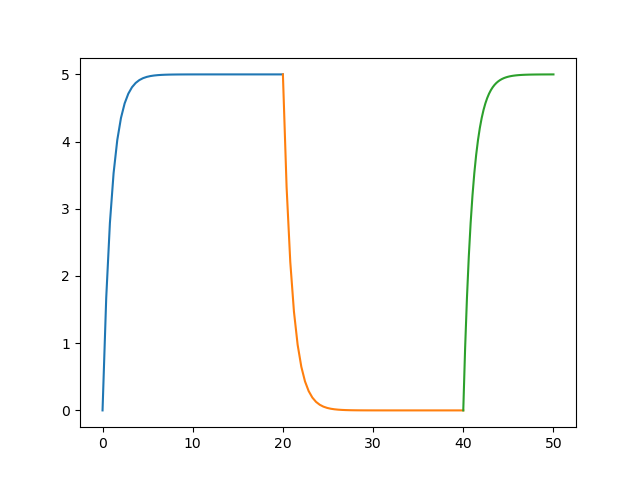
\includegraphics[width=0.8\textwidth]{grafica.png}
    \caption{Grafica de como se comportaria la salida A1 bajo las cirscunstancias planteadas previamente.}
    \label{fig:grafica}
  \end{figure}

\item En este caso usaremos la información que se encontro en la pagina \url{https://es.khanacademy.org/science/electrical-engineering/ee-circuit-analysis-topic/ee-natural-and-forced-response/a/ee-rlc-natural-response-variations} con lo cual sabemos que para detectar el tipo de amortiguamiento que tiene $\alpha$ y $\omega$ en donde
   \begin{align*}
    \alpha &= \frac{R}{2L} \\
    \omega_{0} &= \frac{1}{\sqrt{LC} }
  .\end{align*}

  En donde en este caso quizas lo mas prudente es utilizar equivalencia de fuentes de voltaje a corriente lo que deja las dos resistencias en paralelo y nos permite reducirlas a una sola.
  \begin{align*}
    R = \frac{100 \cdot  2k}{100 + 2k} = 95.23
  .\end{align*}

  por lo tanto, ahora solo queda calcular ambos:
  \begin{align*}
    \alpha &= \frac{95.23}{2\left( 470 \right) } = 0.101\\
    \omega_{0} &= \frac{1}{\sqrt{470} } = 0.046 \\
  .\end{align*}

  por lo tanto $a^2-\omega_0^2$ es mayo que $0$ y por lo tanto sobre amortiguado.
  
\end{enumerate}

\end{document}
